\section{Tree}


\begin{frame}[fragile]{树和二叉树}
  \begin{columns}[T]
    \column{0.5\textwidth}

    树型结构是结点之间有分支,并且具有层次关系的结构,类似于自然界中的树。树有很多
    应用,比如Unix等操作系统中的目录结构。

    \column{0.4\textwidth}
    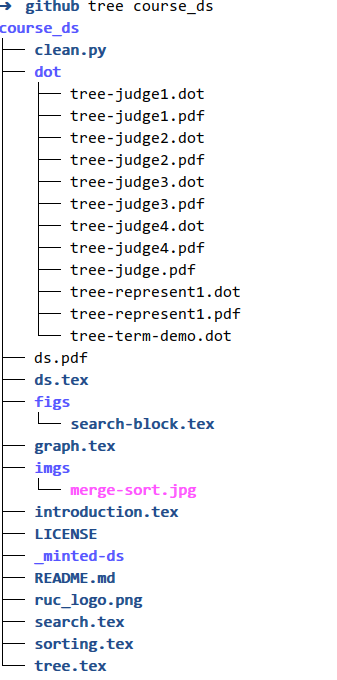
\includegraphics[width=0.9\textwidth]{imgs/linux-tree.png}
  \end{columns}
\end{frame}

\begin{frame}[fragile]
  \frametitle{例子}
\begin{forest}
 [CEO, for tree={rectangle, minimum width=2cm}, fill=red!10
    [CFO [财务人员] ]
    [CTO [工程师] ]
    [CMO [销售人员] ]
 ]
 \node at (current bounding box.south)
 [below=1ex,draw,cloud,aspect=6,cloud puffs=30]
 {\emph{Simple Company Hierarchy}};
\end{forest}
\end{frame}

\begin{frame}[fragile, plain]
  \scalebox{0.7}{
    \begin{forest}
      [学院, for tree={draw=none, rectangle, minimum width=1cm}, fill=red!10, circle
       [社会学部, grow=west [信息资源管理学院, fill=red!10] [新闻学院] [农业与农村发展学院] [社会与人口学院]
       [公共管理学院] [教育学院]]
       [$\cdots$]
       [ 人文学部,grow=east [哲学院] [文学院] [历史学院] [国学院] [艺术学院] [外国语学院] [清史研究所]]
       ]
       \node at (current bounding box.south)
       [below=1ex,draw,cloud,aspect=6,cloud puffs=30]
       {\emph{人民大学学院设置}};
    \end{forest}
  }
\end{frame}

\begin{frame}[fragile]{内容}
  \begin{easylist} \easyitem
    & 树的基本术语
    & 二叉树
    & 遍历二叉树与线索二叉树
    & 树和森林
    & 哈夫曼树
  \end{easylist}
\end{frame}

\subsection{基本术语}

\begin{frame}[fragile]
  \frametitle{树(TREE)}树(Tree)是$n(n \geq 0)$个结点的有限集$T$。 $T$为空时称为空
  树。当$n>0$时,树有且仅有一个特定的称为根(Root)的结点,其余结点可分为$m(m \geq
  0)$个互不相交的子集$T_1, T_2, \cdots, T_m$,其中每个子集又是一棵树,称为子
  树(Subtree)。
  \begin{columns}[T]
    \column{0.55\textwidth}
    \begin{enumerate}
    \item 各子树是互不相交的集合。
    \item 除根结点,其它结点有唯一前驱。
    \item   一个结点可以有零个或多个后继。
    \end{enumerate}

    \column{0.4\textwidth}
    \begin{forest}
      [R, for tree={color=white,fill=black}, fill=red!85
      [A [C] [D] [E]]
      [B [F]]
      ]
    \end{forest}
  \end{columns}
\end{frame}

\begin{frame}[fragile]
  \frametitle{判断哪些是树结构}
  \includegraphics[width=0.3\textwidth]{dot/tree-judge1.pdf} ~~~~~
  \pause
  \includegraphics[width=0.4\textwidth]{dot/tree-judge2.pdf}
\end{frame}

\begin{frame}[fragile]
  \frametitle{判断哪些是树结构}
  \includegraphics[width=0.35\textwidth]{dot/tree-judge3.pdf} ~~~~~
  \pause
  \includegraphics[width=0.4\textwidth]{dot/tree-judge4.pdf}
\end{frame}

\begin{frame}[fragile]
  \frametitle{树的表示形式}
  \includegraphics[width=0.36\textwidth]{dot/tree-represent1.pdf}  \pause
  \scalebox{0.75}{
    \begin{tikzpicture}[b/.style={fill=black!50},n/.style={minimum width=1cm}]
      \draw node[n] (a) {A} node[b, right=0 of a, minimum width=5cm, fill=red!50]{};	

      \draw node[minimum width=0.5cm, below=0.1 of a](bh){} 
      node[n, right=0 of bh] (b) {B} node[b,fill=blue!50, minimum width=4.3cm,right=0 of b]{};	

      \draw node[minimum width=2cm, below=0.2 of bh](dh){} 
      node[n, right=0 of dh] (d) {D} node[b, minimum width=3.5cm,right=0 of d]{};	

      \draw node[minimum width=3.5cm, below=0.2 of dh](ih){} 
      node[n, right=0 of ih] (i) {I} node[b, fill=green!50, minimum width=2.8cm,right=0 of i]{};	

      \draw node[minimum width=3.5cm, below=0.2 of ih](jh){} 
      node[n, right=0 of jh] (j) {J} node[b, fill=green!50, minimum width=2.8cm,right=0 of j]{};	

      \draw node[minimum width=2cm, below=1.2 of dh](eh){} 
      node[n, right=0 of eh] (e) {E} node[b, minimum width=3.5cm,right=0 of e]{};	

      \draw node[minimum width=2cm, below=1.8 of dh](fh){} 
      node[n, right=0 of fh] (f) {F} node[b, minimum width=3.5cm,right=0 of f]{};		


      \draw node[minimum width=0.5cm, below=3.2 of a](ch){} 
      node[n, right=0 of ch] (c) {C} node[b, fill=blue!50, minimum width=4.3cm,right=0 of c]{};	

      \draw node[minimum width=2cm, below=2.8 of dh](gh){} 
      node[n, right=0 of gh] (g) {G} node[b, minimum width=3.5cm,right=0 of g]{};	
      \draw node[minimum width=2cm, below=3.2 of dh](hh){} 
      node[n, right=0 of hh] (h) {H} node[b, minimum width=3.5cm,right=0 of h]{};	

      \draw node[below=0.1 of h] {凹入表表示法};
    \end{tikzpicture}
  } \pause
  
  \begin{columns}[T]
    \begin{column}{0.4\textwidth}
      \centering
      \vspace{2cm}
      (A(B(D(I,J),E, F),C(G,H)))
      
      广义表表示 \\
      
      \pause
    \end{column}
    \begin{column}{0.5\textwidth}
\scalebox{0.65}{
    \begin{tikzpicture}[n/.style={ellipse,draw}]
      \draw node[n, minimum width=7.8cm, minimum height=3.5cm, fill=red!5]{}
      node[n, minimum width=4.5cm, minimum height=2.5cm, xshift=-1.2cm, fill=blue!5]{}
      node[n, minimum width=2.5cm, minimum height=1.8cm, xshift=2.5cm, fill=blue!5]{}
      node[n, minimum width=2cm, minimum height=1.8cm, xshift=-2cm, fill=yellow!5]{}
      node[n, circle,xshift=-2.5cm, fill=green!5]{I}
      node[n, circle,xshift=-1.7cm, fill=green!5]{J}
      node[n, circle,xshift=-0.5cm, fill=yellow!5]{E}
      node[n, circle,xshift=0.4cm, fill=yellow!5]{F}
      node[n, circle,xshift=2cm, fill=yellow!5]{G}
      node[n, circle,xshift=3cm, fill=yellow!5]{H}
      node[yshift=1.35cm]{A}
      node[xshift=-0.8cm,yshift=0.8cm]{B}
      node[xshift=2.5cm, yshift=0.6cm]{C}
      node[xshift=-2cm,yshift=0.6cm]{D};
      \draw node[yshift=-2.2cm] {嵌套集合表示};
    \end{tikzpicture}
  }
  
    \end{column}
  \end{columns}
\end{frame}

\begin{frame}[fragile]
  \frametitle{基本术语}
  \begin{columns}[t]
    \begin{column}{0.5\textwidth}
      \begin{itemize}
      \item 树(tree)
      \item 子树(sub-tree)
      \item 结点(node)
      \item 结点的度(degree)
      \item 叶子(leaf)
      \item 孩子(child)
      \item 父亲(parents)
      \item 兄弟(sibling)
      \item 祖先
      \item 子孙
      \end{itemize}
    \end{column}
    \begin{column}{0.5\textwidth}
      \begin{itemize}
      \item 树的度(degree)
      \item 结点的层次(level)
      \item 树的深度(depth)
      \item 有序树
      \item 无序树
      \item 森林
      \end{itemize}

      \begin{forest}
        [R
        [A, 
        [C] [D]]
        [B [E]]
        ]
      \end{forest}
    \end{column}
  \end{columns}
\end{frame}

\begin{frame}[fragile, plain]
~
\end{frame}

\subsection{二叉树}
\begin{frame}[fragile]
  \frametitle{二叉树(Binary Tree)}
  \begin{itemize}
  \item 二叉树是一种树型结构,它的每个结点至多只有两个子树,分别称为左子树和右子树。
    二叉树是有序树。
  \item 二叉树是$n(n \geq 0)$个结点构成的有限集合。二叉树或为空,或是由一个根结点及
    两棵互不相交的左右子树组成,并且左右子树都是二叉树。
  \item 在二叉树中要区分左子树和右子树,即使只有一棵子树。这是二叉树与树的最主要的
    差别。
  \end{itemize}

  二叉树的一个重要应用是在查找中的应用。当然,它还 有许多与搜索无关的重要应用,比如
  在编译器的设计领域。
\end{frame}

\begin{frame}[fragile]
  \frametitle{二叉树的五种形态}
  \begin{enumerate}
  \item 空二叉树;
  \item 只有根结点(左右子树都为空);
  \item 只有左子树(右子树为空);
  \item 只有右子树(左子树为空);
  \item 左右子树均不空。
  \end{enumerate}

  \scalebox{0.8}{
    \begin{tikzpicture}[n/.style={draw=black!80, thick,fill=black!80, circle, minimum size=0.6cm},
      t/.style={draw=black!80, ellipse, minimum height=2cm,minimum width=1cm, fill=black!20}]
      \draw node[n,dotted, fill=yellow!1] (t1) at (0,0) {};
      \draw[draw=red] (0.5,0.5) -- (-0.5,-0.5);

      \draw node[n] (t2) at (2,0) {};

      \draw node[n] (t3) at (4.5,0) {} node[t, below left=of t3,xshift=0.8cm, rotate=-30] (t31) {};
      \draw[draw] (t3) -- (t31);

      \draw node[n] (t4) at (6.5,0) {} node[t, below right=of t4,xshift=-0.8cm, rotate=30] (t41) {};
      \draw[draw] (t4) -- (t41);

      \draw node[n] (t5) at (11,0) {} node[t, below left=of t5,xshift=0.8cm, rotate=-30] (t51) {} node[t, below right=of t5,xshift=-0.8cm, rotate=30] (t52) {};
      \draw[draw] (t5) -- (t51);
      \draw[draw] (t5) -- (t52);
    \end{tikzpicture}
  }
\end{frame}

\begin{frame}[fragile]
  \frametitle{请观察二叉树, 并回答下列问题}

  \scalebox{0.7} {
    \begin{forest}
      [A, name=A
      [B, name=B [D [H] [I]] [E [J] [K]]]
      [C, name=C [F [L] [M]] [G [N] [O]]]
      ]
     \draw[draw, dotted, thick] (B.north) ++(-2cm, 0.2cm)-- ++(9cm, 0cm)
     node[above, right, yshift=0.5cm]{1};
     \draw[draw, dotted, thick] (B.south) ++(-2cm, -0.2cm)-- ++(9cm, 0cm)
     node[above, right, yshift=0.5cm]{2};
     \draw[draw, dotted, thick] (B.south) ++(-2cm, -1.6cm)-- ++(9cm, 0cm)
     node[above, right, yshift=0.5cm]{3} node[below, right, yshift=-0.5cm] {4};
    \end{forest}
  }

  \begin{enumerate}
  \item 二叉树的第$i$层最多有多少个结点?
  \item 二叉树深度为k,则它最多有多少个结点?
  \item 二叉树有n个节点,请问它最小深度是几?
  \item 二叉树叶子的数目和度为2的节点的数目是否相等?如果不等,又是什么关系?
  \end{enumerate}
\end{frame}

\begin{frame}[fragile]
  \frametitle{二叉树的性质}
  \begin{itemize}
  \item 性质1: 二叉树的第$i$层至多有$2^{i-1}$个结点。
  \item 性质2: 深度为$k$的二叉树至多有$2^k-1$个结点($k \geq 1$)。
  \item \color{red} 性质3: 二叉树中终端结点数为$n_0$,度为2的结点数为$n_2$,则有$n_0 = n_2 + 1$
    (试证明)
  \end{itemize}
\end{frame}

\begin{frame}[fragile]
  \frametitle{二叉树的性质}
  二叉树中终端结点数为$n_0$,度为2的结点数为$n_2$,则有$n_0 = n_2 + 1$

  \begin{columns}[T,c]
    \begin{column}{0.6\linewidth}
      \begin{itemize}
      \item 设二叉树中度为1的结点数为$n_1$, 二叉树中总结点数为$N$,则有:
        
        $N = n_0 + n_1 + n_2$
      \item 再考虑二叉树中的分支数(每个节点有唯一一个入的分支,根节点除外;再考虑出
        的分支数量), 则有:

        $N - 1 =n_1 + 2 \times n_2$
      \item 整理可得:

        $n_0 = n_2 + 1$
      \end{itemize}
    \end{column}
    \begin{column}{0.35\linewidth}      
      \begin{forest}
        [{}, name=root,for tree={color=white,fill=black}
        [{}, name=n21, grow=-55 [{}, name=n31 [{~}] [{~}]]]
        [{}, name=n22, grow=235 [{}, name=n32,[{~}, draw=none,fill=none, no edge] [{~}]]]
        ]
      \end{forest}
    \end{column}
  \end{columns}
\end{frame}

\begin{frame}[fragile]
  \frametitle{完全二叉树}
  \begin{columns}[T]
    \column{0.55\textwidth}
    \begin{forest}
      [1, for tree={font=\scriptsize}
      [2 [4 [8] [9]] [5 [10] [11]]]
      [3 [6 [12] [{}, no edge,draw=none]] [7]]
      ]\
    \end{forest}
    \pause
    
    \column{0.4\textwidth}
    是否完全二叉树?

    \begin{forest}
      [1
      [2 [4] [5]]
      [3 [{}, no edge, draw=none] [7]]
      ]
    \end{forest}

    \pause
    
    \begin{forest}
      [1
      [2]
      [3 [6] [7]]
      ]
    \end{forest}
  \end{columns}
\end{frame}

\begin{frame}[fragile]
  \frametitle{试找出非完全二叉树}

  \begin{forest}
    [{}, for tree={fill=black}]
  \end{forest} \hspace{3cm}
  \begin{forest}
    [{}, for tree={fill=black} [{}] [{}]]
  \end{forest}
  
  \begin{forest}
    [{}, for tree={fill=black}
    [{} [{}] [{}]]
    [{}]]
  \end{forest}
  \begin{forest}
    [{}, for tree={fill=black}
    [{} [{} [{}] [{}]] [{}]]
    [{}]]
  \end{forest}
  \begin{forest}
    [{}, for tree={fill=black}
    [{} [{}] [{}]]
    [{} [{}] [{}]]]
  \end{forest}
  \begin{forest}
    [{}, for tree={fill=black}
    [{} [{} [{} [{}] [{}]] [{}]] [{}]]
    [{}]]
  \end{forest}
  \begin{forest}
    [{}, for tree={fill=black}
    [{} [{} [{}] [{}, no edge, draw=none, fill=none]] [{}]]
    [{} [{}] [{}]]]
  \end{forest}
\end{frame}

\begin{frame}[fragile]
  \frametitle{二叉树的性质}
  \begin{itemize}
  \item 性质4:具有$n$个结点的完全二叉树的深度为:
    \[ \biggl\lfloor {log_2 n} \biggr\rfloor + 1 \] 
  \end{itemize}
  \small
  对于完全二叉树,设深度为$k$, 由$2^{k-1}-1 < n \leq 2^k - 1$可知,
  $2^{k-1} \leq n <2^k$, 则 $k-1 \leq log_2n < k$
  (参考性质2)
  
  \begin{columns}[T]
    \column{0.45\textwidth}
    \scalebox{0.6}{
      \begin{forest}
        [1, for tree={font=\scriptsize}
        [2 [4 [8] [9]] [5 [10] [11]]]
        [3 [6 [12] [13]] [7 [14] [15]]]
        ]
      \end{forest}
    }
    
    满二叉树
    \column{0.45\textwidth}
    \scalebox{0.6}{
      \begin{forest}
        [1, for tree={font=\scriptsize}
        [2 [4 [8] [9]] [5 [10] [11]]]
        [3 [6 [12] [{}, no edge, draw=none]] [7]]
        ]
      \end{forest}
    }
    
    完全二叉树
  \end{columns}
\end{frame}

\begin{frame}[fragile]
  \frametitle{测试}

\begin{columns}[T]
  \column{0.6\textwidth}
    对于完全二叉树:
  \begin{enumerate}
  \item 若完全二叉树有叶子结点出现在第$k$层,它可能还有(~~~~~~)层的叶子结点;
  \item 若某结点的右子树的最大层次为$L$,则其左子树的最大层次为(~~~~~~~~);
  \item 若按如图所示的编号方式,试求出编号为$i$的节点的父节点和子节点的编号.
  \end{enumerate}

  \column{0.36\textwidth}
  \scalebox{0.6}{
    \begin{forest}
      [1
      [2 [4 [8] [9]] [5 [10] [11]]]
      [3 [6 [12] [{}, no edge,draw=none]] [7]]
      ]\
    \end{forest}
  }
\end{columns}

\pause
\begin{enumerate}
\item $k-1$, $k+1$
\item $L$ or $L+1$
\end{enumerate}
\end{frame}


\begin{frame}[fragile]
  \frametitle{二叉树的性质}
  \begin{center}
    \scalebox{0.6} {
      \begin{forest}
        [1, name=A,for tree={}
        [2, name=B [4 [8] [9]] [5 [10] [11]]]
        [3, name=C [6 [12] [{}, no edge,draw=none] ] [7] ]
        ]
        \draw[draw, dotted, thick] (B.north) ++(-2cm, 0.2cm)-- ++(9cm, 0cm)
        node[above, right, yshift=0.5cm]{1};
        \draw[draw, dotted, thick] (B.south) ++(-2cm, -0.2cm)-- ++(9cm, 0cm)
        node[above, right, yshift=0.5cm]{2};
        \draw[draw, dotted, thick] (B.south) ++(-2cm, -1.6cm)-- ++(9cm, 0cm)
        node[above, right, yshift=0.5cm]{3} node[below, right, yshift=-0.5cm] {4};
      \end{forest}
    }
  \end{center}

  \begin{itemize}
  \item 性质5: 对具有$n$个结点的完全二叉树的结点按层次顺序编号,对任意结点$i$有:
    \begin{itemize}
    \item (有关结点$i$的双亲)若$i=1$,则为二叉树的根结点, 没有双亲;否则双亲结点的
      编号为: $\biggl\lfloor{\dfrac{i}{2}}\biggr\rfloor$
    \item (有关结点$i$的孩子) 若$n<2 \cdot i$, 则结点$i$无左孩子;否则左孩子编号
      是$2 \cdot i$。
    \item 若$n<2 \cdot i+1$,则结点i无右孩子;否则右孩子编号为$2 \cdot i+1$
    \end{itemize}
  \end{itemize}
\end{frame}

\begin{frame}[fragile]
  \frametitle{二叉树的存储结构:顺序存储}
  \begin{columns}
    \column{0.45\textwidth}

    \scalebox{0.6} {
      \begin{forest}
        [1, name=A,for tree={color=white,fill=black}
        [2, for tree={dotted,color=black,fill=white}, [4 [8] [9]] [5 [10] [11]]]
        [3, name=C [6 [12] [{}, no edge,draw=none, fill=none] ] [7] ]
        ]
      \end{forest}
    }

    \vspace{2cm}
    \scalebox{0.6}{
      \begin{tikzpicture}[ n/.style={minimum size=0.8cm}]
        \draw node[] (n0) {};
        \foreach \x  [evaluate = \x as \xp using int(\x-1)] in {1, ..., 12}
        \draw node[n, right=0 of n\xp](n\x) {$\xp$};

        \foreach \x in {2,4,5,8,9, ..., 11}
        \draw node[n, above=0 of n\x, draw](d\x) {$\^$};
        \foreach \x/\y in {1/1,3/3,6/6,7/7,12/12}
        \draw node[n, above=0 of n\x, draw,white, fill=black](d\x) {$\y$};
      \end{tikzpicture}
    }

    \column{0.55\textwidth}
    \begin{minted}[bgcolor=yellow!20, fontsize=\scriptsize]{c}
      #define MAX_SIZE 100
      typedef int SqBiTree[MAX_SIZE];
      SqBiTree bt;
    \end{minted}

    \begin{minted}[bgcolor=red!5, fontsize=\scriptsize]{java}
      class SqBiTree {
        //static int MAX_SIZE = 100;
        //int[] data = new int[MAX_SIZE];
        List<Integer> data = new ArrayList<Integer>();
      }
    \end{minted}
  \end{columns}
  
  \begin{itemize}
  \item 把结点安排成一个恰当的序列(编号),存储在数组中
  \item 便于“随机存取”
  \end{itemize}
\end{frame}

\begin{frame}[fragile]
  \frametitle{二叉树的存储结构:顺序存储}
  \begin{itemize}
  \item 适用于完全二叉树
  \end{itemize}

  \begin{columns}
    \column{0.6\textwidth}
    \scalebox{0.8} {
      \begin{forest}
        [$a$, for tree={color=white,fill=black}
        [{}, draw=none, no edge, fill=none]
        [$b$
        [{}, draw=none, no edge, fill=none]
        [$c$ [{}, draw=none, no edge, fill=none] [$d$] ]
        ]
        ]
      \end{forest}
    }

    \column{0.4\textwidth}
    \scalebox{0.8} {
      \begin{forest}
        [1, for tree={color=white,fill=black}
        [2 [4] [5 [6] [7]]]
        [3]
        ]
      \end{forest}
    }
  \end{columns}

  \pause
  
  \hspace{-1cm}
  \scalebox{0.7}{
    \begin{tikzpicture}[ n/.style={minimum size=0.8cm}]
      \draw node[n] (n0) {0};
      \foreach \x  [evaluate = \x as \xp using int(\x-1)] in {1, ..., 14}
      \draw node[n, right=0 of n\xp](n\x) {$\x$};

      \foreach \x in {1,3,4,5,7,8, ..., 13}
      \draw node[n, above=0 of n\x, draw](d\x) {$0$};

      \foreach \x/\y in {0/a,2/b,6/c,14/d}
      \draw node[n, above=0 of n\x, draw, fill=red!10](d\x) {$\y$};
    \end{tikzpicture}
  }

  \pause
  \hspace{4cm}
  \scalebox{0.7}{
    \begin{tikzpicture}[ n/.style={minimum size=0.8cm}]
      \draw node[n] (n0) {0};
      \foreach \x  [evaluate = \x as \xp using int(\x-1)] in {1, ..., 10}
      \draw node[n, right=0 of n\xp](n\x) {$\x$};

      \foreach \x in {5, ..., 8}
      \draw node[n, above=0 of n\x, draw](d\x) {$0$};

      \foreach \x/\y in {0/1,1/2,2/3,3/4,4/5,9/6,10/7}
      \draw node[n, above=0 of n\x, draw, fill=red!10](d\x) {$\y$};
    \end{tikzpicture}
  }
\end{frame}

\begin{frame}[fragile]
  \frametitle{二叉树的链式存储:二叉链表}
  \begin{columns}[T]
    \column{0.4\textwidth}
    \scalebox{0.7}{
      \begin{forest}
        [1
        [2 [{}, no edge, draw=none] [4 [5] [6]]]
        [3]]
      \end{forest}
    }
    \column{0.4\textwidth}
    \includegraphics[width=0.6\textwidth]{dot/tree-store-bilink.pdf}
  \end{columns}

  \small
  \begin{columns}
    \column{0.48\textwidth}
    \begin{minted}[fontsize=\scriptsize,bgcolor=red!5]{c}
      typedef struct BiTNode  { // C Code
        ElemType data;
        struct BiTNode *lchild, *rchild;
      } BiTNode, *BiTree;
    \end{minted}

    \column{0.48\textwidth}
    \begin{minted}[fontsize=\scriptsize,bgcolor=yellow!10]{c}
      class BiTNode<T> { //Java Code
        T data;
        BiTNode lchild, rchild;
      }
    \end{minted}
  \end{columns}

  思考:含$n$个结点的二叉链表中有多少个空指针?

  \pause
  指针域一共有$2*n$个,分支共有$N-1$,  每个分支占用一个指针域,所以空指针数量为:  $2*n - (n-1) = n+1$
\end{frame}

\begin{frame}[fragile]
  \frametitle{二叉树的链式存储:三叉链表}
  \begin{itemize}
  \item 二叉链表不便查找父节点, 可加一个指向双亲的指针
  \end{itemize}

  \begin{columns}[T]
    \column{0.5\textwidth}
    \scalebox{0.5}{
      \begin{forest}
        [1
        [2 [{}, no edge, draw=none] [4 [5] [6]]]
        [3]]
      \end{forest}
    }
    \includegraphics[width=0.8\textwidth]{dot/tree-store-trilink.pdf}
    
    \column{0.5\textwidth}
    \begin{minted}[fontsize=\scriptsize,bgcolor=red!5]{c}
      typedef struct BiTNode  { // C Code
        ElemType data;
        struct BiTNode *lchild, *rchild, *parent;
      } BiTNode, *BiTree;
    \end{minted}

    \begin{minted}[fontsize=\scriptsize,bgcolor=yellow!10]{c}
      class BiTNode<T> { //Java Code
        T data;
        BiTNode lchild, rchild, parent;
      }
    \end{minted}
  \end{columns}

  思考: 有n个结点的三叉链表有多少个空指针?

  \pause
  \scriptsize
  对于二叉链表,指针域一共有$2*n$个,分支共有$N-1$,  每个分支占用一个指针域,所以空指针数量为$2*n - (n - 1) = n+1 $;  对于parent,根节点无父节点,所以共有$n+1+1=n+2$个空指针
\end{frame}

\begin{frame}[fragile, plain]
  ~  
\end{frame}


\subsection{遍历二叉树和线索二叉树}
\begin{frame}[fragile]
  \frametitle{遍历二叉树和线索二叉树}

  在二叉树的一些应用中,常常要求在树中查找具有某种特征的结点,或者对树中全部结点逐
  一进行某种处理。这就引入了遍历二叉树的问题,即如何按某条搜索路径巡访树中的每一个
  结点,使得每一个结点均被访问一次且仅访问一次。
\end{frame}

\begin{frame}[fragile]
  \frametitle{二叉树的遍历}
 \begin{itemize}
 \item 遍历是指按某种方式访问所有结点,使每个结点被访问一次且只被访问一次。
 \item 二叉树的遍历是按一定规则将二叉树的结点排成一个线性序列,即非线性序列线性
   化。
 \item 遍历的方式: 深度优先和广度优先,深度优先又分为三种:
   \begin{itemize}
   \item 先序次序
   \item 中序次序(对称序次序)
   \item 后序次序 
   \end{itemize}
 \end{itemize} 
\end{frame}

\begin{frame}[fragile]
  \frametitle{二叉树的遍历}
  \begin{easylist}
    & 1、先序遍历二叉树的操作定义为: 若二叉树为空,则空操作;否则
    && (1)访问根结点;
    && (2)先序遍历左子树;
    && (3)先序遍历右子树。
    & 2、中序遍历二叉树的操作定义为:若二叉树为空,则空操作;否则
    && (1)中序遍历左子树;
    && (2)访问根结点;
    && (3)中序遍历右子树。
    & 3、后序遍历二叉树的操作定义为:若二叉树为空,则空操作;否则
    && (1)后序遍历左子树;
    && (2)后序遍历右子树;
    && (3)访问根结点。
  \end{easylist}
\end{frame}

\begin{frame}[fragile]
  \frametitle{示例}
  \scalebox{0.8}{
    \begin{forest}
      [A
      [B [D] [{}, no edge, draw=none]]
      [C [E [{}, no edge, draw=none] [G]] [F [H] [I]]]
      ]
    \end{forest}
  }

  \pause
  \begin{itemize}
  \item 先序:ABDCEGFHI
  \item 中序:DBAEGCHFI
  \item 后序:DBGEHIFCA
  \item 广度优先:ABCDEFGHI
  \end{itemize}
\end{frame}

\begin{frame}[fragile]
  \frametitle{二叉树的遍历}
  \begin{columns}[T]
    \column{0.6\textwidth}
    //先序遍历二叉树递归算法C伪代码
    \begin{minted}[bgcolor=red!5, fontsize=\small]{c}
      status preOrderTraverse(BiTree T){
        if(T){
          printf(T->data);
          preOrderTraverse(T->lchild);
          preOrderTraverse(T->rchild);
        }
      }
    \end{minted}
    \begin{itemize}
    \item status代表什么?
    \item printf代表什么?
    \end{itemize}

    \column{0.4\textwidth}
    \scalebox{0.8}{
      \begin{forest}
        [A
        [B [D] [{}, no edge, draw=none]]
        [C [E [{}, no edge, draw=none] [G]] [F [H] [I]]]
        ]
      \end{forest}
    }    
  \end{columns}
\end{frame}


\begin{frame}[fragile]
  \frametitle{二叉树的遍历}
  \begin{columns}[T]
    \column{0.6\textwidth}
    先序遍历递归算法的Java实现
  
    \begin{minted}[bgcolor=yellow!10,fontsize=\small]{java}
      class Node {
        String data;
        Node left, right;
      }
      class Tree {
        void preOrderTraverse(Node node) {
          if(node != null) {
            System.out.println(node.data);
            preOrderTraverse(node.left);
            preOrderTraverse(node.right);
          }
        }
      }
    \end{minted}

    \column{0.4\textwidth}
    \scalebox{0.8}{
      \begin{forest}
        [A
        [B [D] [{}, no edge, draw=none]]
        [C [E [{}, no edge, draw=none] [G]] [F [H] [I]]]
        ]
      \end{forest}
    }
  \end{columns}
\end{frame}

\begin{frame}[fragile, allowframebreaks]
  \frametitle{中序遍历的Java实现}
  \begin{minted}[fontsize=\scriptsize]{java}
    public class Tree {
      Node root;

      public Tree(Node root) {
        this.root = root;
      }

      void inOrderTraverse() {
        inOrderTraverse(root);
      }

      void inOrderTraverse(Node node) {
        if(node != null) {
          inOrderTraverse(node.lc);
          //visit(node);
          System.out.println(node);
          inOrderTraverse(node.rc);
        }
      }

      public static void main(String[] args) {
        Node a  =new Node("A",
        new Node("B", new Node("D"), null),
        new Node("C", new Node("E"), new Node("F"))
        );
        Tree tree = new Tree(a);
        tree.inOrderTraverse();
      }

      static class Node {
        String data;
        Node lc, rc;

        public Node(String data, Node lc, Node rc) {
          this.data = data;
          this.lc = lc;
          this.rc = rc;
        }

        public Node(String data) {
          this.data = data;
          this.lc = null;
          this.rc = null;
        }

        public String toString(){
          return data;
        }
      }
    }
  \end{minted}
\end{frame}
\begin{frame}[fragile]
  \frametitle{如下将得到树的什么序列?}
  \begin{columns}[T]
    \column{0.6\textwidth}
    \begin{minted}[bgcolor=yellow!10,fontsize=\small]{c}
      status traverse(BiTree T) {
        InitStack(S);
        p = T;
        while(p || !StackEmpty(S)) {
          if(p) {
            push(S, p); p = p->lchild;
          } else {
            pop(S, p);
            printf(p->data);
            p = p->rchild;
          }
        }
        return OK;
      }
    \end{minted}

    \column{0.4\textwidth}
    \scalebox{0.8}{
      \begin{forest}
        [A
        [B [D] [{}, no edge, draw=none]]
        [C [E [{}, no edge, draw=none] [G]] [F [H] [I]]]
        ]
      \end{forest}
    }
  \end{columns}  
\end{frame}

\begin{frame}[fragile]
  \frametitle{二叉树的遍历:广度优先}
  \begin{columns}[T]
    \column{0.6\textwidth}
    算法步骤:
    \begin{itemize}
    \item 访问节点
    \item 从左到右依次访问儿子节点
    \item 重复前一步骤
    \end{itemize}
    
    \begin{tikzpicture}[ n/.style={minimum width=1cm,minimum height=0.6cm, draw}]
      \draw node[] (n0) {};
      \foreach \x  [evaluate = \x as \xp using int(\x-1)] in {1, ..., 7}
      \draw node[n, right=0 of n\xp](n\x) {};
      
      \draw node[n, right=0 of n0] {A};
    \end{tikzpicture}

    \begin{tikzpicture}[ n/.style={minimum width=1cm,minimum height=0.6cm, draw}]
      \draw node[] (n0) {};
      \foreach \x  [evaluate = \x as \xp using int(\x-1)] in {1, ..., 7}
      \draw node[n, right=0 of n\xp](n\x) {};
      
      \draw node[n, right=0 of n1] {B} node[n, right=0 of n2]{C};
    \end{tikzpicture}

    \begin{tikzpicture}[ n/.style={minimum width=1cm,minimum height=0.6cm, draw}]
      \draw node[] (n0) {};
      \foreach \x  [evaluate = \x as \xp using int(\x-1)] in {1, ..., 7}
      \draw node[n, right=0 of n\xp](n\x) {};
      
      \draw node[n, right=0 of n2] {C} node[n, right=0 of n3]{D};
    \end{tikzpicture}

    .......

    课堂练习:编程实现广度优先遍历。
    
    \column{0.4\textwidth}
    \scalebox{0.8}{
      \begin{forest}
        [A
        [B [D] [{}, no edge, draw=none]]
        [C [E [{}, no edge, draw=none] [G]] [F [H] [I]]]
        ]
      \end{forest}
    }
  \end{columns}
  
\end{frame}

\begin{frame}[fragile]
  \frametitle{补充}
  \begin{itemize}
  \item 由一棵给定的二叉树可以获得三种遍历序列,同样,也可以由这些遍历序列来重新构
    造二叉树。
  \item 举例
    
    先序:ABCDEFGHIJ
    
    中序:CBDEAFHIGJ
  \item 由于不能从遍历序列中区分二叉树的左、右子树,因此单用一个遍历序列是无法构造
    二叉树的。利用中序遍历序列,并结合先序遍历序列或后序遍历序列就能重新构造二叉
    树。
  \end{itemize}
\end{frame}

\begin{frame}[fragile]
  \frametitle{二叉树的线索化}
  \begin{itemize}
  \item 基于二叉链表可以很方便地查找节点的左、右孩子。
  \item 问题:如何快速查找给定结点在遍历所得线性序列中的前驱和后继。
  \item 该信息在遍历的动态过程中才能得到。如果经常需要查找前驱和后继,需要在二叉链
    表的结点上添加指向前驱和后继的指针,叫做{\color{red}线索}。这样得到的二叉树称
    为{\color{red}线索二叉树}。
  \end{itemize}
\end{frame}

\begin{frame}[fragile]
  \frametitle{举例:中序线索二叉树}
  \includegraphics[width=0.6\textwidth]{dot/tree-thread.pdf}
  \begin{itemize}
  \item 以右图二叉树为例,中序序列为(~~~~~~~~~~~).
  \item 线索的表示:若结点有左子树,则指向其左孩子,否则指向其前驱;若节点有右子树,则指向
    其右孩子,否则指向其后继。
  \item 请问结点A和F的前驱和后继分别是?
  \end{itemize}
\end{frame}

\begin{frame}[fragile]
  \frametitle{举例:中序线索二叉树}
  \includegraphics[width=0.9\textwidth]{dot/tree-thread2.pdf}
\end{frame}

\begin{frame}[fragile]
  \frametitle{带头节点的中序线索链表}
  参照双向链表,在二叉树线索链表上添加头节点,令头节点的左孩子指向二叉树的根节点。
  优点:既可从第一个结点起顺后继遍历,也可从最后一个结点起顺前驱遍历。
  
  \includegraphics[width=0.7\textwidth]{dot/tree-thread3.pdf}
\end{frame}

\begin{frame}[fragile]
  \frametitle{练习}
  画出下图的先序、中序和后序线索二叉树。

  \begin{forest}
    [A
    [B [D [{}, no edge, draw=none] [G]] [{}, no edge, draw=none]]
    [C [E] [F]]
    ]
  \end{forest}
\end{frame}

\begin{frame}[fragile, plain]
  ~  
\end{frame}

\subsection{树和森林}
\begin{frame}[fragile]
  \frametitle{树和森林}
  \begin{itemize}
  \item 树的存储结构
  \item 树和二叉树的转换
  \item 森林和二叉树的转换
  \item 树和森林的遍历
  \end{itemize}
\end{frame}

\begin{frame}[fragile]
  \frametitle{树的存储结构:双亲表示法}
  \begin{columns}[T]
    \column{0.5\textwidth}
    \begin{forest}
      [R, for tree={edge={draw, <-}} [A [C] [D] [E]] [B [F]]]
    \end{forest}

    \vspace{1cm}
    \scalebox{0.6}{
      \begin{tikzpicture}[ n/.style={minimum size=0.8cm}]
        \draw node[n] (n0) {结点索引} node[n,above=0 of n0](label) {标记} node[n,above=0 of label,xshift=-0.5cm] {父结点索引};
        \foreach \x  [evaluate = \x as \xp using int(\x-1)] in {1, ..., 7}
        \draw node[n, right=0 of n\xp](n\x) {$\xp$};

        \foreach \x/\y in {1/R,2/A,3/B,4/C, 5/D, 6/E, 7/F}
        \draw node[n, above=0 of n\x, draw](n\x) {$\y$};

        \foreach \x/\y in {1/{-},2/0,3/0,4/1, 5/1, 6/1, 7/2}
        \draw node[n, above=0 of n\x, draw](n\x) {$\y$};
      \end{tikzpicture}
    }

    \column{0.5\textwidth}

    \begin{minted}[bgcolor=red!5, fontsize=\scriptsize]{java}
      class PtNode<T> {
        T data;
        int parent;
      }
    \end{minted}

    \begin{minted}[bgcolor=yellow!10, fontsize=\scriptsize]{c}
      typedef struct{
        telemtype data;
        int parent;
      } PtNode;
    \end{minted}
    
    因节点的度各异,从父亲指向孩子极不方便!若经常需要查找孩子结点,双亲表示法就不方
    便了。
  \end{columns}
\end{frame}

\begin{frame}[fragile]
  \frametitle{树的存储结构:孩子表示法}
  \begin{columns}[T]
    \column{0.5\textwidth}
    \scalebox{0.7}{
      \begin{forest}
        [R, for tree={edge={draw, <-}} [A [C] [D] [E]] [B [F]]]
      \end{forest}
    }

    \small 把每个结点的孩子结点排列成一个线性表,以单链表做存储结构.

    \scalebox{0.6}{
      \begin{tikzpicture}[ n/.style={minimum height=0.8cm, minimum width=1cm},
        n2/.style={minimum height=0.6cm, minimum width=1cm, fill=red!5},
        e/.style={->, very thick}]
        \draw node[n] (n0) {索引} node[n,right=0 of n0](label) {标记/父结点};
        \foreach \x  [evaluate = \x as \xp using int(\x-1)] in {1, ..., 7}
        \draw node[n, below=0 of n\xp](n\x) {$\xp$};

        \foreach \x/\y/\z in {1/R/,2/A/,3/B/,4/C/$\wedge$, 5/D/$\wedge$, 6/E/$\wedge$, 7/F/$\wedge$}
        \draw node[n, right=0 of n\x, draw, fill=yellow!10](\y) {$\y$} node[n, right=0 of \y, draw] (P\y) {\z};

        \draw node[n2, draw, right=of PR] (c11) {1} node[n2, draw, right=0 of c11] (c12) {};
        \draw node[n2, draw, right=of c12] (c21) {2} node[n2, draw, right=0 of c21] (c22) {$\wedge$};
        \draw[e] (PR.center) -- (c11) (c12.center)--(c21);				

        \draw node[n2, draw, right=of PA] (c11) {3} node[n2, draw, right=0 of c11] (c12) {};
        \draw node[n2, draw, right=of c12] (c21) {4} node[n2, draw, right=0 of c21] (c22) {};
        \draw node[n2, draw, right=of c22] (c31) {5} node[n2, draw, right=0 of c31] (c32) {$\wedge$};

        \draw[e] (PA.center) -- (c11) (c12.center)--(c21) (c22.center)--(c31);				

        \draw node[n2, draw, right=of PB] (c11) {6} node[n2, draw, right=0 of c11] (c12) {$\wedge$};
        \draw[e] (PB.center) -- (c11);
      \end{tikzpicture}
    }

    \column{0.5\textwidth}

    试写出ChildNode, CTree \pause
    
    \begin{minted}[bgcolor=red!5, fontsize=\scriptsize]{java}
      class TNode<T> {
        T data;
        ChildNode firstChild;
      }
      
      class ChildNode<T> {
        int index;
        ChildNode nextSibling;
      }

      class Tree {
        TNode<String>[] nodes = new TNode<String>[]{new TNode("R"), new TNode("A")};
        TNode root = nodes[0];
      }
    \end{minted}
  \end{columns}
\end{frame}

\begin{frame}[fragile]
  \frametitle{树的存储结构:双亲+孩子表示法}

  \scalebox{0.7}{
    \begin{forest}
      [R, for tree={edge={draw, <-}} [A [C] [D] [E]] [B [F]]]
    \end{forest}
  }

  \scalebox{0.6}{
    \begin{tikzpicture}[ n/.style={minimum height=0.8cm, minimum width=1cm},
      n2/.style={minimum height=0.6cm, minimum width=1cm, fill=red!5},
      e/.style={->, very thick}]
      \draw node[n] (n0) {索引} node[n,right=0 of n0](label) {标记/父结点};
      \foreach \x  [evaluate = \x as \xp using int(\x-1)] in {1, ..., 7}
      \draw node[n, below=0 of n\xp](n\x) {$\xp$};

      \foreach \x/\y/\t/\z in {1/R/-1/,2/A/0/,3/B/0/,4/C/1/$\wedge$, 5/D/1/$\wedge$, 6/E/1/$\wedge$, 7/F/2/$\wedge$}
      \draw node[n, right=0 of n\x, draw, fill=yellow!10](\y) {$\y$} 
      node[n, right=0 of \y, draw, fill=red!20] (T\y) {\t}
      node[n, right=0 of T\y, draw] (P\y) {\z};

      \draw node[n2, draw, right=of PR] (c11) {1} node[n2, draw, right=0 of c11] (c12) {};
      \draw node[n2, draw, right=of c12] (c21) {2} node[n2, draw, right=0 of c21] (c22) {$\wedge$};
      \draw[e] (PR.center) -- (c11) (c12.center)--(c21);				

      \draw node[n2, draw, right=of PA] (c11) {3} node[n2, draw, right=0 of c11] (c12) {};
      \draw node[n2, draw, right=of c12] (c21) {4} node[n2, draw, right=0 of c21] (c22) {};
      \draw node[n2, draw, right=of c22] (c31) {5} node[n2, draw, right=0 of c31] (c32) {$\wedge$};

      \draw[e] (PA.center) -- (c11) (c12.center)--(c21) (c22.center)--(c31);				

      \draw node[n2, draw, right=of PB] (c11) {6} node[n2, draw, right=0 of c11] (c12) {$\wedge$};
      \draw[e] (PB.center) -- (c11);
    \end{tikzpicture}
  }

\end{frame}

\begin{frame}[fragile]
  \frametitle{树的存储结构:孩子兄弟表示法}

  试想如何借鉴二叉树的存储方法?

  树和森林的存储结构与算法都很复杂,如果能够将它们转换为二叉树,不但可以采用二叉树
  的存储结构,而且可以利用二叉树的有关算法来实现有关操作。幸运的是,树或森林与二叉
  树之间存在一一对应关系。
\end{frame}

\begin{frame}[fragile]
  \frametitle{树的存储结构:孩子兄弟表示法}
  使用二叉链表, 两个指针分别指向第一个孩子和下一个兄弟.
  
  \begin{minted}[bgcolor=red!5, fontsize=\scriptsize]{java}
    class CSNode<T> {
      T data;
      CSNode<T> firstChild, nextSibling;
    }  
  \end{minted}

  \begin{columns}[T]
    \column{0.2\textwidth}
    ~
    
    \column{0.3\textwidth}
    \scalebox{0.7}{
      \begin{forest}
        [R [A [C] [D] [E]] [B [F]]]
      \end{forest}
    }

    \column{0.2\textwidth}
    \vspace{1cm} {\Huge{$\Rightarrow$}}

    \column{0.3\textwidth}
    \scalebox{0.7}{
      \begin{forest}
        [R
        [A
        [C [{}, no edge, draw=none] [D [{},no edge, draw=none] [E]]]
        [B [F] [{}, no edge, draw=none]]]
        [{}, no edge, draw=none]]
      \end{forest}
    }
  \end{columns}
\end{frame}

\begin{frame}[fragile]
  \frametitle{树与二叉树的转换}
  \begin{itemize}
  \item 孩子作左子树的根,兄弟作右子树的根
  \item 任何一棵树对应的二叉树,其右子树必空,也就是说,所有的树都可以转化为二叉
    树,但不是所有的二叉树都可以转化为树。
  \end{itemize}

  \begin{columns}[T]
    \column{0.2\textwidth}
    ~
    \column{0.3\textwidth}
    \scalebox{0.7}{
      \begin{forest}
        [A [B] [C] [D]]
      \end{forest}
    }

    \column{0.2\textwidth}
    \vspace{1cm} {\Huge{$\Leftrightarrow$}}

    \column{0.3\textwidth}
    \scalebox{0.7}{
      \begin{forest}
        [A
        [B [{}, no edge, draw=none] [C [{},no edge, draw=none] [D]]]
        [{}, no edge, draw=none]]
      \end{forest}
    }
  \end{columns}
\end{frame}

\begin{frame}[fragile]
  \frametitle{森林与二叉树的转换}
  \begin{itemize}
  \item 零棵或有限棵不相交的树的集合称为森林。自然界中树和森林是不同的概念,但在数
    据结构中,树和森林只有很小的差别——任何一棵树,删去根结点就变成了森林。
  \item 根据树的二叉链表表示,任何一棵和树对应的二叉树的右子树必空。若将森林中第二
    棵树的根结点看成第一棵树的根结点的兄弟,则可以导出森林和二叉树的对应关系。
  \end{itemize}
\end{frame}

\begin{frame}[fragile]
  \frametitle{森林与二叉树的转换示例}
  \begin{columns}[T]
    \column{0.6\textwidth}
  \scalebox{0.8}{
  \begin{tabular}{c c c}
    \begin{forest}
      [A [C] [D] [E]]
    \end{forest} &
    \begin{forest}
      [B [F]]
    \end{forest} &
    \begin{forest}
      [G [H] [I [J]]]
    \end{forest} \\
    \huge{$\downarrow$} & \huge{$\downarrow$} & \huge{$\downarrow$}  \\
    \begin{forest} 
      [A [C [{}, no edge, draw=none] [D [{}, no edge, draw=none] [E]]] [{}, no edge, draw=none]]
    \end{forest} &
    \begin{forest}
      [B [F] [{}, no edge, draw=none]]
    \end{forest} &
    \begin{forest}
      [G [H [{}, no edge, draw=none] [I [J] [{}, no edge, draw=none]]] [{}, no edge, draw=none]]
    \end{forest}
  \end{tabular}
  }

  \column{0.4\textwidth}
  \pause
  \scalebox{0.7}{
    \begin{forest}
      [A
      [C [{}, no edge, draw=none] [D [{}, no edge, draw=none] [E]]]
      [B [F]  [G [H [{}, no edge, draw=none] [I [J] [{}, no edge, draw=none]]] [{}, no edge, draw=none]]]]
    \end{forest}
  }
  \end{columns}
\end{frame}

\begin{frame}[fragile]
  \frametitle{树和森林的遍历}
  \small
  请按下述原则写出该树的遍历序列
  \begin{itemize}
  \item 先根遍历: =相应二叉树的先序遍历
    
    首先访问根结点;再从左到右遍历根结点的每一棵子树。

  \item 后根遍历: =相应二叉树的中序遍历

    首先 按照从左到右的顺序后根遍历根结点的每一棵子树,再访问根结点。
    
  \end{itemize}

  请画出该树对应的二叉树,并写出该二叉树的先、中、后序遍历

  \begin{columns}[T]
    \column{0.4\textwidth}
    \hspace{1cm}
    \scalebox{0.8} {
      \begin{forest}
        [A [B [E] [F]] [C] [D [G]]]
      \end{forest}
    }
    \column{0.6\textwidth}
    \pause
    上图的先根遍历序列为:A B E F C D G \\
    上图的后根遍历序列为:E F B C G D A
  \end{columns}
\end{frame}

\begin{frame}[fragile]
  \frametitle{森林的遍历}
  \small
  \begin{easylist}
    & 前序遍历(相应二叉树的先序遍历)
    && 访问森林中第一棵树的根结点;
    && 先根遍历第一棵树的根结点的子树;
    && 先根遍历去掉第一棵树后的子森林。
    & 中序遍历(相应二叉树的中序遍历)
    && 后根遍历第一棵树的根结点的子树;
    && 访问森林中第一棵树的根结点;
    && 后根遍历去掉第一棵树后的子森林。
  \end{easylist}

  \begin{columns}
    \column{0.5\textwidth}
    \scalebox{0.6}{
      \begin{tabular}{c c c}
        \begin{forest}
          [A [B]]
        \end{forest} &
                       \begin{forest}
                         [C [D] [E] [F]]
                       \end{forest} &
                                      \begin{forest}
                                        [G [H [J]] [I [K]]]
                                      \end{forest}
      \end{tabular}
    }

    \column{0.5\textwidth}
    前序遍历结果: A B C D E F G H J I K
    
    中序遍历结果:B A D E F C J H K I G
  \end{columns}
\end{frame}

\begin{frame}[fragile, plain]
  ~  
\end{frame}

\subsection{哈夫曼树}
\begin{frame}[fragile]
  \frametitle{哈夫曼树}
  \small
  \begin{itemize}
  \item Huffman coding (哈夫曼编码) 是David A. Huffman于1952年在麻省理工攻读博士
    时发明的一种编码方法,可用于无损数据压缩的熵编码。 Huffman编码广泛应用在涉及数
    字压缩和传输的领域,如fax、modem、计算机网络和HDTV。
  \item 原理:使用一张特殊的编码表将源字符进行编码,它的特殊之处在于它是根据每一个
    源字符出现的估算概率建立起来的——出现概率高的字符使用较短的编码,反之出现概率低
    的则使用较长的编码,使编码后的字符串的平均期望长度降低,从而达到无损压缩数据的
    目的。若能比较准确的估计英文中各个字母出现概率,就能大幅提高无损压缩的效率。
  \item 例如,在英文中,用普通的表示方法时,每个英文字母均占用一个字节(byte),即8位。
    实际上,e的出现概率很高,而z的出现概率则最低。当利用哈夫曼编码进行压缩时,e可能
    用1位来表示,z可能用25位。
  \end{itemize}
\end{frame}

\begin{frame}[fragile]
  \frametitle{David Huffman (1925/08/09 -- 1999/10/07)}
  \begin{itemize}
  \item 1950年,Huffman在MIT的信息理论与编码研究生班学习。Robert Fano教授让学生们
    自己决定是参加期未考试还是做一个大作业,因为大作业比期末考试可能更容易通
    过,Huffman选择了后者。正是一个大作业促使了Huffman算法的诞生!
  \item 离开MIT后,Huffman来到University of California, Santa Cruz的计算机系任
    教,并为此系的学术做出了许多杰出的工作。而他的算法也广泛应用于传真机,图象压缩
    和计算机安全领域。但是Huffman却从未为此算法申请专利或其它能够为他带来经济利益
    的东西,他将他全部的精力放在教学上,用他自己的话来说,“My products are my
    students.”
  \item David Huffman对于有限状态自动机,开关电路,异步过程和信号设计也做出了杰出贡
    献。
  \end{itemize}
\end{frame}

\begin{frame}[fragile]
  \frametitle{举例:假设学生成绩分布如下,试构造一棵树}
  \begin{tabular}{|c|c|c|c|c|c|}
    \hline
    Grade & Bad & Pass & General & Good & Excellent \\ \hline
    Score & 0 -- 59 & 60 -- 69 & 70 -- 79 & 80 -- 89 & 90 -- 100 \\ \hline
    Ratio & 0.05 & 0.15 & 0.40 & 0.30 & 0.10 \\ \hline
  \end{tabular}

  \scalebox{0.6}{
    \begin{forest}
      [$s<60$, for tree={draw=none}
      [Bad,,edge label={node[midway,right,font=\scriptsize]{Y}}]
      [$s<70$,edge label={node[midway,right,font=\scriptsize]{N}} [Pass] [$s<80$ [General] [$s<90$ [Good] [Excellent]]]]
      ]
    \end{forest}
  }
  \scalebox{0.7}{
    \begin{forest}
      [$s<80$, for tree={draw=none}
      [$s<70$,edge label={node[midway,right,font=\scriptsize]{Y}} [$s<60$ [Bad]
      [Pass]] [General]]
      [$s<90$,edge label={node[midway,right,font=\scriptsize]{N}} [Good] [Excellent] ]]
    \end{forest}
  }
  Which one is better?
\end{frame}

\begin{frame}[fragile, plain]

  \begin{tabular}{|c|c|c|c|c|c|}
    \hline
    Grade & Bad & Pass & General & Good & Excellent \\ \hline
    Score & 0 -- 59 & 60 -- 69 & 70 -- 79 & 80 -- 89 & 90 -- 100 \\ \hline
    Ratio & 0.05 & 0.15 & 0.40 & 0.30 & 0.10 \\ \hline
  \end{tabular}

  \begin{columns}[T]
    \column{0.25\textwidth}
    \scalebox{0.6}{
      \begin{forest}
        [$s<60$, for tree={draw=none}
        [Bad,,edge label={node[midway,right,font=\scriptsize]{Y}}]
        [$s<70$,edge label={node[midway,right,font=\scriptsize]{N}} [Pass] [$s<80$ [General] [$s<90$ [Good] [Excellent]]]]
        ]
      \end{forest}
    }

    \column{0.75\textwidth}
    \begin{itemize}
    \item 结点的带权路径程度(Weighted Path Length):

      \[WPL(good) = 4*0.3=1.2 \]
      
    \item 树的带权路径长度:
      \begin{equation*}
        \begin{array}{r c l}
          WPL(TREE) & = & 1 \times 0.05  \\
          & & + 2 \times 0.15 \\
          & & + 3 \times 0.40 \\
          & & + 4 \times \times 0.30 \\
          & & + 5 \times 0.10 \\
          & = & 3.15 \\
        \end{array}
      \end{equation*}
    \end{itemize}
  \end{columns}
\end{frame}

\begin{frame}[fragile]
  \frametitle{练习:求树的带权路径长度}

  \begin{center}
    \begin{tabular}{|c|c|c|c|c|c|}
      \hline
      Grade & Bad & Pass & General & Good & Excellent \\ \hline
      Score & 0 -- 59 & 60 -- 69 & 70 -- 79 & 80 -- 89 & 90 -- 100 \\ \hline
      Ratio & 0.05 & 0.15 & 0.40 & 0.30 & 0.10 \\ \hline
    \end{tabular}
    
    \scalebox{0.6}{
      \begin{forest}
        [$s<60$, for tree={draw=none}
        [Bad,,edge label={node[midway,right,font=\scriptsize]{Y}}]
        [$s<70$,edge label={node[midway,right,font=\scriptsize]{N}} [Pass] [$s<80$ [General] [$s<90$ [Good] [Excellent]]]]
        ]
      \end{forest}
    }
  \end{center}
\end{frame}

\begin{frame}[fragile]
  \frametitle{哈夫曼树}具有最小带权路径长度的二叉树称为哈夫曼树(最优二叉树)。

  \begin{columns}[T]
    \column{0.55\textwidth}
    \scalebox{0.6}{
      \begin{forest}        
        [{} [{} [2] [3]] [{} [4] [7]]]       
      \end{forest}
    }

    $WPL=2\times 2 + 2\times 3 + 2 \times 4 + 2 \times 7 = 32$

    \scalebox{0.6}{
      \begin{forest}
        [{} [2] [{} [3] [{} [4] [7]]]]       
      \end{forest}
    }

    $WPL=1 \times 2 + 2\times 3 + 3 \times 4 + 3 \times 7 = 41$
    
    \column{0.55\textwidth}
    \pause
    \scalebox{0.8}{
      \begin{forest}
        [{} [7] [{} [4] [{} [3] [2]]]]
      \end{forest}
    }
    
    $WPL=1\times 7 + 2 \times 4 + 3 \times 3 + 3 \times 2 = 30$
  \end{columns}
\end{frame}


\begin{frame}[fragile]
  \frametitle{哈夫曼树的构造}

  由给定的$n$个权值$\{w_1, w_2, \cdots, w_n\}$,构造$n$棵只有一个叶子结点的二叉
  树 , 从而得到一个二叉树的集合$F=\{T_1, T_2, \cdots, T_n\}$.

  \begin{enumerate}
  \item 在$F$中选取根结点的权值最小和次小的两棵二叉树作为左、右子树构造一棵新的二叉
    树,这棵新的二叉树根结点的权值为其左、右子树根结点权值之和;
  \item 在集合$F$中删除作为左、右子树的两棵二叉树,并将新建立的二叉树加入到集合
    $F$中;
  \item 重复(2)、(3)两步,当$F$中只剩下一棵二叉树时,这棵二叉树便是所要建立的哈夫曼
    树。
  \end{enumerate}
\end{frame}

\begin{frame}[fragile]
  \frametitle{例子}
  1, 3, 5, 7
\end{frame}

\begin{frame}[fragile]
  \frametitle{课堂作业}
  \begin{columns}
    \column{0.3\textwidth}
    \scalebox{0.6}{
      \begin{forest}
        [A
        [B [D] [{}, no edge, draw=none]]
        [C [E [{}, no edge, draw=none] [G]] [F [H] [I]]]
        ]
      \end{forest}
    }

    \begin{minted}{java}
      class TNode {
        String data;
        int lc, rc;
      }
    \end{minted}

    \column{0.3\textwidth}
    \begin{tabular}{c | c | c | c|}
      \hline
      0 & A & 1 & 2 \\ \hline
      1 & B & 3 & -1 \\ \hline
      2 & C & 4 & 5 \\ \hline
      3 & D & -1 & -1 \\ \hline
      4 & E & -1 & 6 \\ \hline
      5 & F & 7 & 8 \\ \hline
      6 & G & -1 & -1 \\ \hline
      7 & H & -1 & -1 \\ \hline
      8 & I & -1 & -1 \\ \hline
    \end{tabular}

    \column{0.4\textwidth}
    \begin{itemize}
    \item 给定树$T$如图所示, 请写递归程序实现如下功能:
    \item (1)遍历树T,显示其先序/中序/后序 序列;
    \item (2)求结点数、叶子数;
    \item (3)求树T的深度.
    \end{itemize}
  \end{columns}
\end{frame}

\begin{frame}[fragile]
  \frametitle{本章作业}
  哈夫曼编码

  \begin{easylist}
    &   根据26个英文字母的频度,为每一个字母赋予一个唯一的最优编码

    & 输出要求, 每行一个字母,及其对应编码,如:

    && A: 00100
    && B: 0001
    && ...
  \end{easylist}
\end{frame}


\begin{frame}[fragile]
  \frametitle{英文字母的频率表}

  \begin{tabular}{|c | c || c | c || c | c| }
    \hline
    字母	& 出现频率 &	字母	& 出现频率	& 字母	& 出现频率 \\ \hline
    a	& 8.167\% &	j	& 0.153\% &	s	& 6.327\% \\ \hline
    b	& 1.492\% &	k	& 0.772\% &	t	& 9.056\% \\ \hline
    c	& 2.782\% &	l	& 4.025\% &	u	& 2.758\% \\ \hline
    d	& 4.253\% &	m	& 2.406\% &	v	& 0.978\% \\ \hline
    e	& 12.702\% &	n	& 6.749\% &	w	& 2.360\% \\ \hline
    f	& 2.228\% &	o	& 7.507\% &	x	& 0.150\% \\ \hline
    g	& 2.015\% &	p	& 1.929\% &	y	& 1.974\% \\ \hline
    h	& 6.094\% &	q	& 0.095\% &	z	& 0.074\% \\ \hline
    i	& 6.966\% &	r	& 5.987\% &    ~ & 		\\ \hline
  \end{tabular}
\end{frame}